\documentclass[a4paper]{article}
\usepackage{amsmath, amssymb, amsfonts}
\usepackage[margin=1in]{geometry}
\usepackage{graphicx}
\usepackage{tikz}
\usepackage{esint}
\setlength{\parindent}{0em}
\setlength{\parskip}{1ex}
\newcommand{\vct}[1]{\overrightarrow{#1}}
\newcommand{\dif}{\mathrm{d}}
\newcommand{\pd}[2]{\frac{\partial {#1}}{\partial {#2}}}
\newcommand{\dd}[2]{\frac{\mathrm{d} {#1}}{\mathrm{d} {#2}}}
\newcommand{\C}{\mathbb{C}}
\newcommand{\R}{\mathbb{R}}
\newcommand{\Q}{\mathbb{Q}}
\newcommand{\Z}{\mathbb{Z}}
\newcommand{\N}{\mathbb{N}}
\newcommand{\fn}[3]{{#1}\colon {#2} \rightarrow {#3}}
\newcommand{\avg}[1]{\langle {#1} \rangle}
\newcommand{\Sum}[2][0]{\sum_{{#2} = {#1}}^{\infty}}
\newcommand{\Lim}[1]{\lim_{{#1} \rightarrow \infty}}
\newcommand{\Binom}[2]{\begin{pmatrix} {#1} \cr {#2} \end{pmatrix}}

\begin{document}
\paragraph{Naloga.} Poišči biholomorfno $F:\{z\in\C\colon\,\left|z+1\right|<\sqrt{2}\}\cup\{z\in\C\colon\,\left|z+1\right|<\sqrt{2}\}\,\to\,D(0,1)$ \\
\begin{figure}[h!]
    \centering
    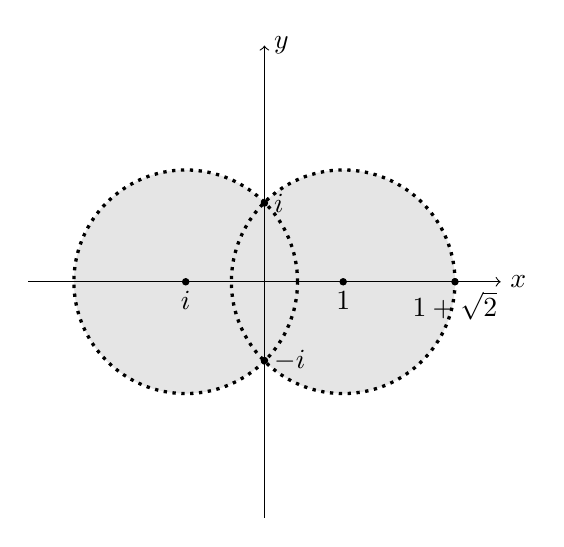
\begin{tikzpicture}
        \fill[gray!20] (-1, 0) circle (1.42);
        \fill[gray!20] (1, 0) circle (1.42);
        \draw[dotted, very thick] (1, 0) circle (1.42);
        \draw[dotted, very thick] (-1, 0) circle (1.42);
        \draw[->] (-3, 0) -- (3, 0) node[right] {$x$};
        \draw[->] (0, -3) -- (0, 3) node[right] {$y$};
        \filldraw (0, 1) circle (0.04) node[right] {$i$};
        \filldraw (0, -1) circle (0.04) node[right] {$-i$};
        \filldraw (1, 0) circle (0.04) node[below] {$1$};
        \filldraw (-1, 0) circle (0.04) node[below] {$i$};
        \filldraw (2.42, 0) circle (0.04) node[below] {$1 + \sqrt{2}$};
    \end{tikzpicture}
\end{figure}
\newline
Vidimo, ali pa izračunamo, da je kot v stičišču pri $-i$ enak $3\pi/2$. Poskusimo torej ta dva kroga preslikati v prve tri kvadrante:
\begin{align*}
    -i & \mapsto 0 \\
    i & \mapsto \infty \\
    1 + \sqrt{2} & \mapsto 3 \\
\end{align*}
Vemo, da bo imela takšna preslikava obliko
$$f(z) = \frac{az + b}{cz + d}$$
Iz zahtev $f(-i) = 0$ in $f(i) = \infty$ dobimo
$$b = ai,~~d = -ci$$
Nazadnje izrazimo $a$:
$$(1 + \sqrt{2})a + ia = 3((1 + \sqrt{2})c - ic)$$
$$a = \frac{3(1 + \sqrt{2} - i)}{1 + \sqrt{2} + i}\,c$$
Sledi: $\displaystyle{f(z) = 3\frac{1 + \sqrt{2} - i}{1 + \sqrt{2} - i} \,\frac{z + i}{z - i}}$
\newline
\begin{figure}[h!]
    \centering
    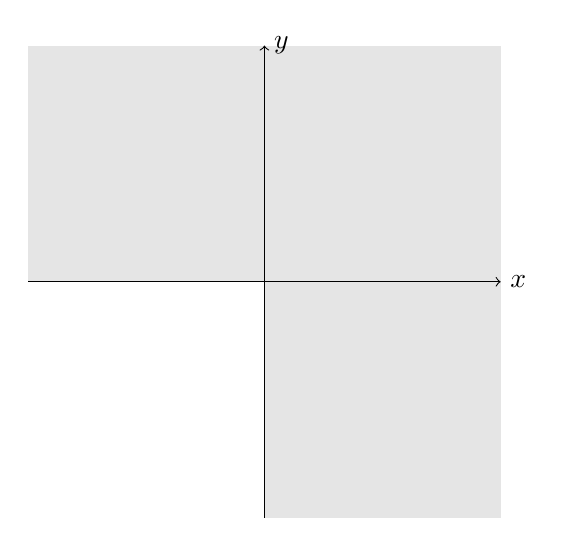
\begin{tikzpicture}
        \fill[gray!20] (0, 0) rectangle (3, -3);
        \fill[gray!20] (0, 0) rectangle (3, 3);
        \fill[gray!20] (0, 0) rectangle (-3, 3);
        \draw[->] (-3, 0) -- (3, 0) node[right] {$x$};
        \draw[->] (0, -3) -- (0, 3) node[right] {$y$};
    \end{tikzpicture}
\end{figure}
\newline
Nazadnje uporabimo funkcijo $z^{2/3}$, da dobljeno območje preslikamo v zgornjo polravnino, nato pa uporabimo že znano Möbiusovo preslikavo
$$\varphi(z) = \frac{z - i}{- z - i},$$
da to preslikamo v odprti krog.
\newpage
\paragraph{Dirichletov problem.} Funkcija $\fn{u}{\mathcal{D}}{\R}$ je harmonična, če velja $\displaystyle{\Delta u = \pd{^2u}{x^2} + \pd{^2u}{y^2} = 0}$. Pri tem je $\mathcal{D}$ zaprta podmnožica $\R^2$.
Dirichletov problem: Najti takšno funkcijo $u$, ki bo harmonična na $\mathcal{D}$, na $\mathcal{\partial D}$ pa zavzame vrednosti funkcije $f$. \\
Problem rešimo z Greenovo funkcijo $\fn{G}{\overline{\mathcal{D}} \times \mathcal{D}}{\R}$, ki naj ima dve lastnosti:
\begin{enumerate}
    \item $G(\vct{r}, \vct{r_0}) = 0 ~~ \forall\vct{r}\in\partial\mathcal{D}$
    \item $\Delta_{\vct{r}} G(\vct{r}, \vct{r_0}) = \delta(\vct{r} - \vct{r_0})$
\end{enumerate}
Nekoliko priročnejša verzija teh zahtev (vsaj pri vajah) je
\begin{enumerate}
    \item $G(\vct{r}, \vct{r_0}) = 0 ~~ \forall\vct{r}\in\partial\mathcal{D}$
    \item $G(\vct{r}, \vct{r_0}) = \frac{1}{2\pi}\ln\left|\vct{r} - \vct{r_0}\right| + \varphi(\vct{r}, \vct{r_0})$, pri čemer bodi $\varphi$ harmonična.
\end{enumerate}
Greenova funkcija hkrati reši Poissonov problem:
$$\Delta u = f(x,y),~~~u\Big|_{\partial\mathcal{D}} = 0$$
Njena rešitev je $$u(\vct{r_0}) = \iint_{\mathcal{D}} f(\vct{r})G(\vct{r},\vct{r_0})\,\dif x\,\dif y$$
\paragraph{Naloga.} Bodi $\mathcal{D} = \{(x, y) \in \R^2\colon~y>0\}$. Poišči Greenovo funkcijo območja $D$. \\[3mm]
Vemo, da bo imela Greenova formula obliko
$$G(\vct{r}, \vct{r_0}) = \frac{1}{2\pi}\ln\left|\vct{r}-\vct{r_0}\right|+\varphi(\vct{r},\vct{r_0})$$
Izberemo $\vct{r_0} = (x_0,\,y_0)$. Če jo prezrcalo+imo čez os $y=0$, dobimo $\vct{r_1} = (x_0,\,-y_0)$
Greenova funkcija za tako območje je $\displaystyle{G(\vct{r}, \vct{r_0}) = \frac{1}{2\pi}\ln\left|\vct{r} - \vct{r_0}\right| - \frac{1}{2\pi}\ln\left|\vct{r} - \vct{r_1}\right|}$
To storimo zato, da funkcija konvergira proti 0, če pošljemo $y_0$ proti $0$ (tj. če se $\vct{r_0}$ približuje robu območja.)
\paragraph{Naloga.} Poišči Greenovo funkcijo območja $\mathcal{D} = \{(x, y)\in\R^2\colon~x,y>0\}$
\begin{figure}[h!]
    \centering
    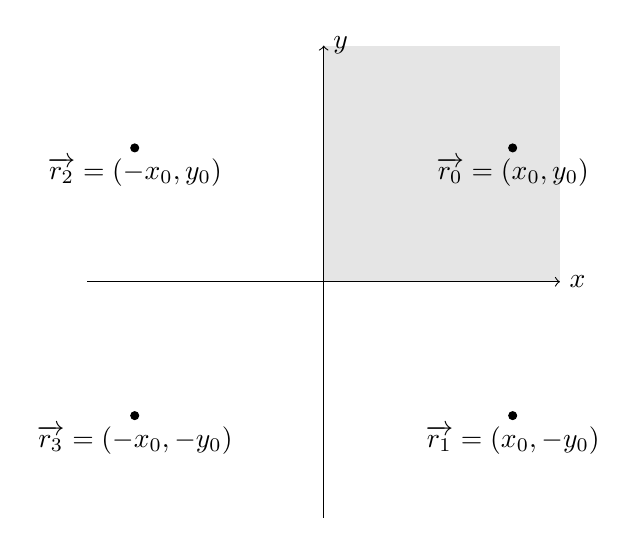
\begin{tikzpicture}
    \fill[gray!20] (0, 0) rectangle (3, 3);
    \draw[->] (-3, 0) -- (3, 0) node[right] {$x$};
    \draw[->] (0, -3) -- (0, 3) node[right] {$y$};
    \filldraw (2.4, 1.7) circle (0.05) node[below] {$\vct{r_0} = (x_0, y_0)$};
    \filldraw (-2.4, 1.7) circle (0.05) node[below] {$\vct{r_2} = (-x_0, y_0)$};
    \filldraw (2.4, -1.7) circle (0.05) node[below] {$\vct{r_1} = (x_0, -y_0)$};
    \filldraw (-2.4, -1.7) circle (0.05) node[below] {$\vct{r_3} = (-x_0, -y_0)$};
    \end{tikzpicture}
\end{figure}
\newpage
Spet pričakujemo, da bo Greenova funkcija oblike
$$G(\vct{r}, \vct{r_0}) = \frac{1}{2\pi} \ln\left|\vct{r}-\vct{r_0}\right| + \varphi(\vct{r}, \vct{r_0})$$
Spet bomo naredili isto kot prej, in sicer moramo poskrbeti, da bo $G$ na robu območja zavzela vrednost 0. Izkaže se, da ni dovolj odšteti le $\displaystyle{\frac{1}{2\pi}\ln\left|\vct{r} - \vct{r_1}\right|}$ in $\frac{1}{2\pi}\ln\left|\vct{r} - \vct{r_2}\right|$. Velja torej
$$G(\vct{r}, \vct{r_0}) = \frac{1}{2\pi}\ln\left|\vct{r} - \vct{r_0}\right| - \frac{1}{2\pi}\ln\left|\vct{r} - \vct{r_1}\right| - \frac{1}{2\pi}\ln\left|\vct{r} - \vct{r_2}\right| - \frac{1}{2\pi}\ln\left|\vct{r} - \vct{r_3}\right|$$
Preveriti moramo le, da je funkcija $\varphi$ harmonična na $\mathcal{D}$ (to velja, saj ima singularnosti le v $\vct{r_1},\,\vct{r_2}$ in $\vct{r_3}$, ki ne ležijo na območju $\mathcal{D}$). Nazadnje preverimo, ali je $G(\vct{r}, \vct{r_0}) = 0~\forall\vct{r}\in\partial\mathcal{D}$.
To storimo tako, da jo izvrednotimo v poljubnih točkah $\vct{r} = (x, 0)$ in $\vct{r} = (0, y)$.
\end{document}